\begin{figure}
\centering
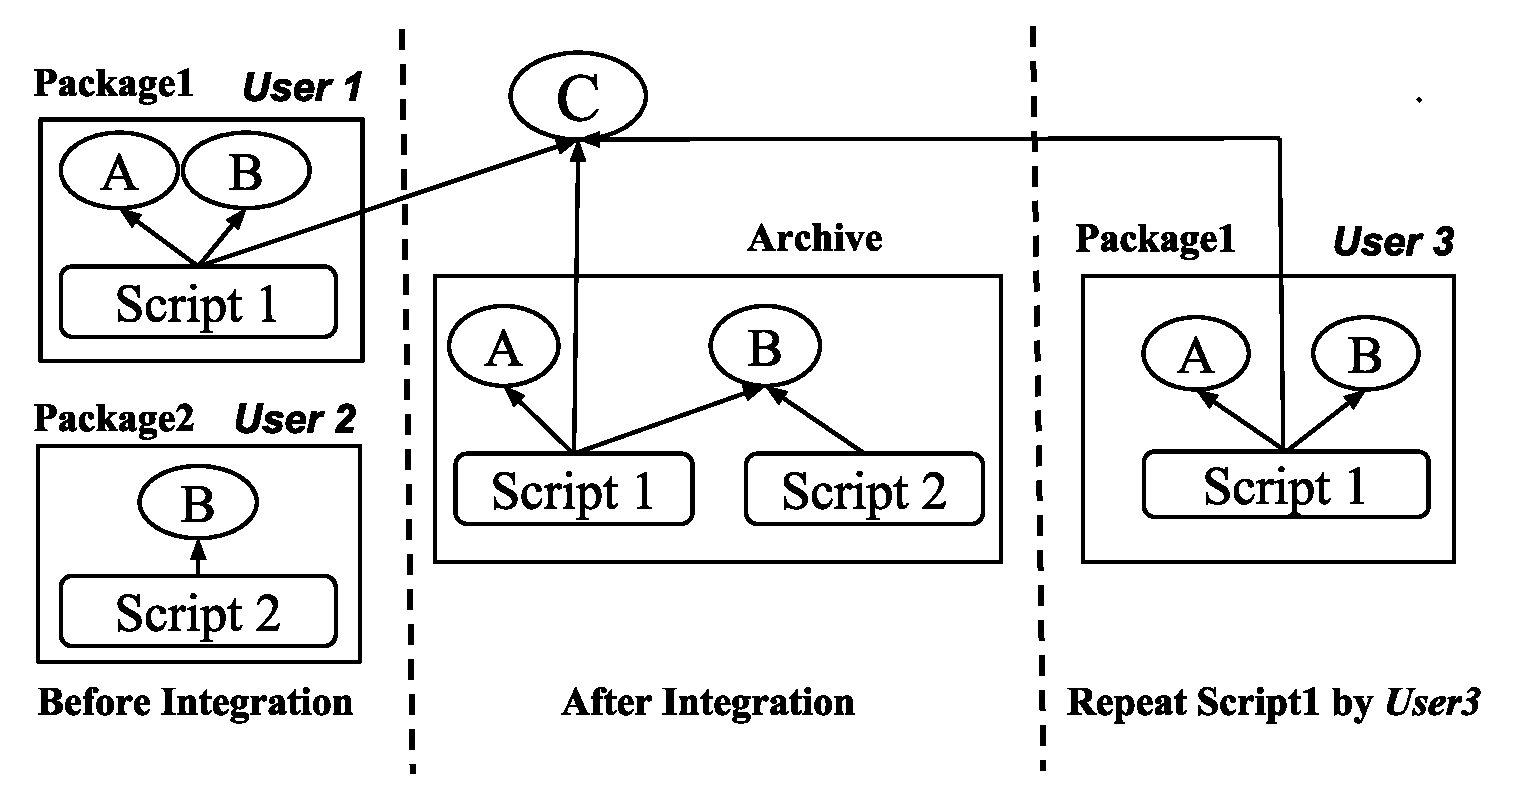
\includegraphics[width=.6\textwidth]{preservation-integration.eps}
\caption{Preserving Multiple Artifacts}
\label{fig:Preservation integration}
\end{figure}

\section{Open Problems}

Figure~\ref{fig:Preservation integration} shows the rough information
architecture of the archive that we imagine for complex
scientific software like TauRoast.
Each artifact to be preserved is a package that consists of a top-level
script to invoke the software, a dependency map, and the dependencies
themselves, which may be external to the original program.  The artifacts
are then ingested into the archive, where shared dependencies are stored
only once.  In cases where an artifact has a dependency on a trusted
(or very large) remote archive, the dependency may simply be tracked
. A researcher that wishes to reproduce a given
result need only refer to the unique identifier of the artifact, and will
be able to automatically extract all of the dependent components of
that artifact.

For example, in Figure~\ref{fig:Preservation integration} Script 1 depends on items A, B, and C.  Items A and B are ingested into the archive, where B is shared with Script 2.  Item C is stored in another trustworthy repository and is tracked rather than ingested.  When Script 1 is exported from the repository, items A and B are exported along with it, while C can be copied or remain remote, according to the end user's choice.

As simple as that picture appears, there are a number of problems that must be solved to get there:

{\bf Measure the Mess or Force Cleanliness?}  Two radically different approaches to dependency tracking are possible.  The first is to allow end users complete freedom to construct their environment as desired, then \emph{measure} what items were actually used.  As we have shown, this is possible, but has significant overheads and does not fully preserve the structure or intent of the end user.   The second approach is to \emph{force} users to work in a clean environment in which no resource can be used until a proper dependency has been declared.  This ensures that all dependencies are known in advance (and made explicit to the end user) but places a variety of restrictions on the user's daily work, and may prevent creative approaches that do not fit within the curator's view of how programs should be structured.  Whether end users will accept the inconvenience of forced cleanliness for the benefits of reproducibility can only be discovered through experiment.

{\bf Granularity of Dependencies.}  Dependencies could be handled
at many different levels of granularity.  In this work, we have shown
how they can be handled at the level of entire repositories or individual files.
Other possible choices might include intermediate-sized software packages
(like RPM) or in the case of experimental data, even portions of individual large files.  Clearly, a larger granularity will result in 
simpler dependency maps, and more wasted space; smaller granularity results
in complex dependency maps and less wasted space.  A hybrid solution may
be able to combine both by storing large granularity dependencies, but
selecting sub-items out of objects when efficiency demands it.

{\bf Scope of Reuse.}  We have presented the data preservation
problem as primarily one of accurate reproduction: if a result depends
on running program X, we must be able to run exactly X again.  However,
the goal of scientific reproducibility is rarely limited to running
\emph{precisely} what a predecessor did. Often, the objective is to
change a parameter or a data input in order to see how the result is affected.
To that end, the preservation system must capture enough of the surrounding
material to permit modifications to succeed.  From this perspective,
a larger granularity of preservation is desirable.  A better understanding of
how end users will consume preserved software will help to shape how
software is preserved in the first place.

{\bf Dependency Detection.}  If we allow users to work in uncontrolled
environments, then we must have better methods for understanding the dependencies  of existing programs.  At first, we relied on an expert reader to examine
the user's script and extract the dependencies.  This is clearly
not a scalable approach.  We then demonstrated an automated method of observing
what individual files are accessed by a program. However, this does
not cover all types of dependencies, particularly those that are networked.
More sophisticated observation techniques could infer higher-level information,
such as the RPM package names of the files accessed, the URLs of remote
repositories named throughout the program, or even the addresses and names of networked dependencies like databases and filesystems.

{\bf Source, Binary, or Both?}  A science archive might choose to retain
the source code of an artifact or the binary code that can actually run in a given environment.
While conventional wisdom suggests that access to source code is critical for the long term
survival and evolution of a piece of software, it also requires the maintenance of an enormous
amount of supporting software in the form of compilers, linkers, and supporting libraries for
the target platform.  Rebuilding all of these for every invocation of an artifact is
likely to have excessive cost.  We suggest that a realistic repository will have to
maintain \emph{both}: the source describes the ultimate meaning of the code, but
the binary is an important performance cache, a backup if the compiler toolchain should
fail to be preserved, and a checksum to ensure that a source artifact was rebuilt correctly.

